\documentclass[]{article}
\usepackage{graphicx}

%opening
\title{Assignment 1 CDA}
\author{Tim van Rossum, 4246306\\
	Michiel Doesburg,}

\begin{document}

\maketitle

\section{A visualization of the data}
For the visualization part of this assignment, we first started out by making bar plots of different kinds, but eventually settled  for the scatterplot as seen in figure 1. This scatterplot uses the amount of Eurocent spent per transaction, to allow for better comparisons to be made, as there were five different currencies in the dataset. As can be seen from the scatterplot, there are basically no fraudulent transactions where more than 800 Euro was spent, while there are benign transactions where more than 800 Euro was spent.
\begin{figure}[h!]
	\centering
	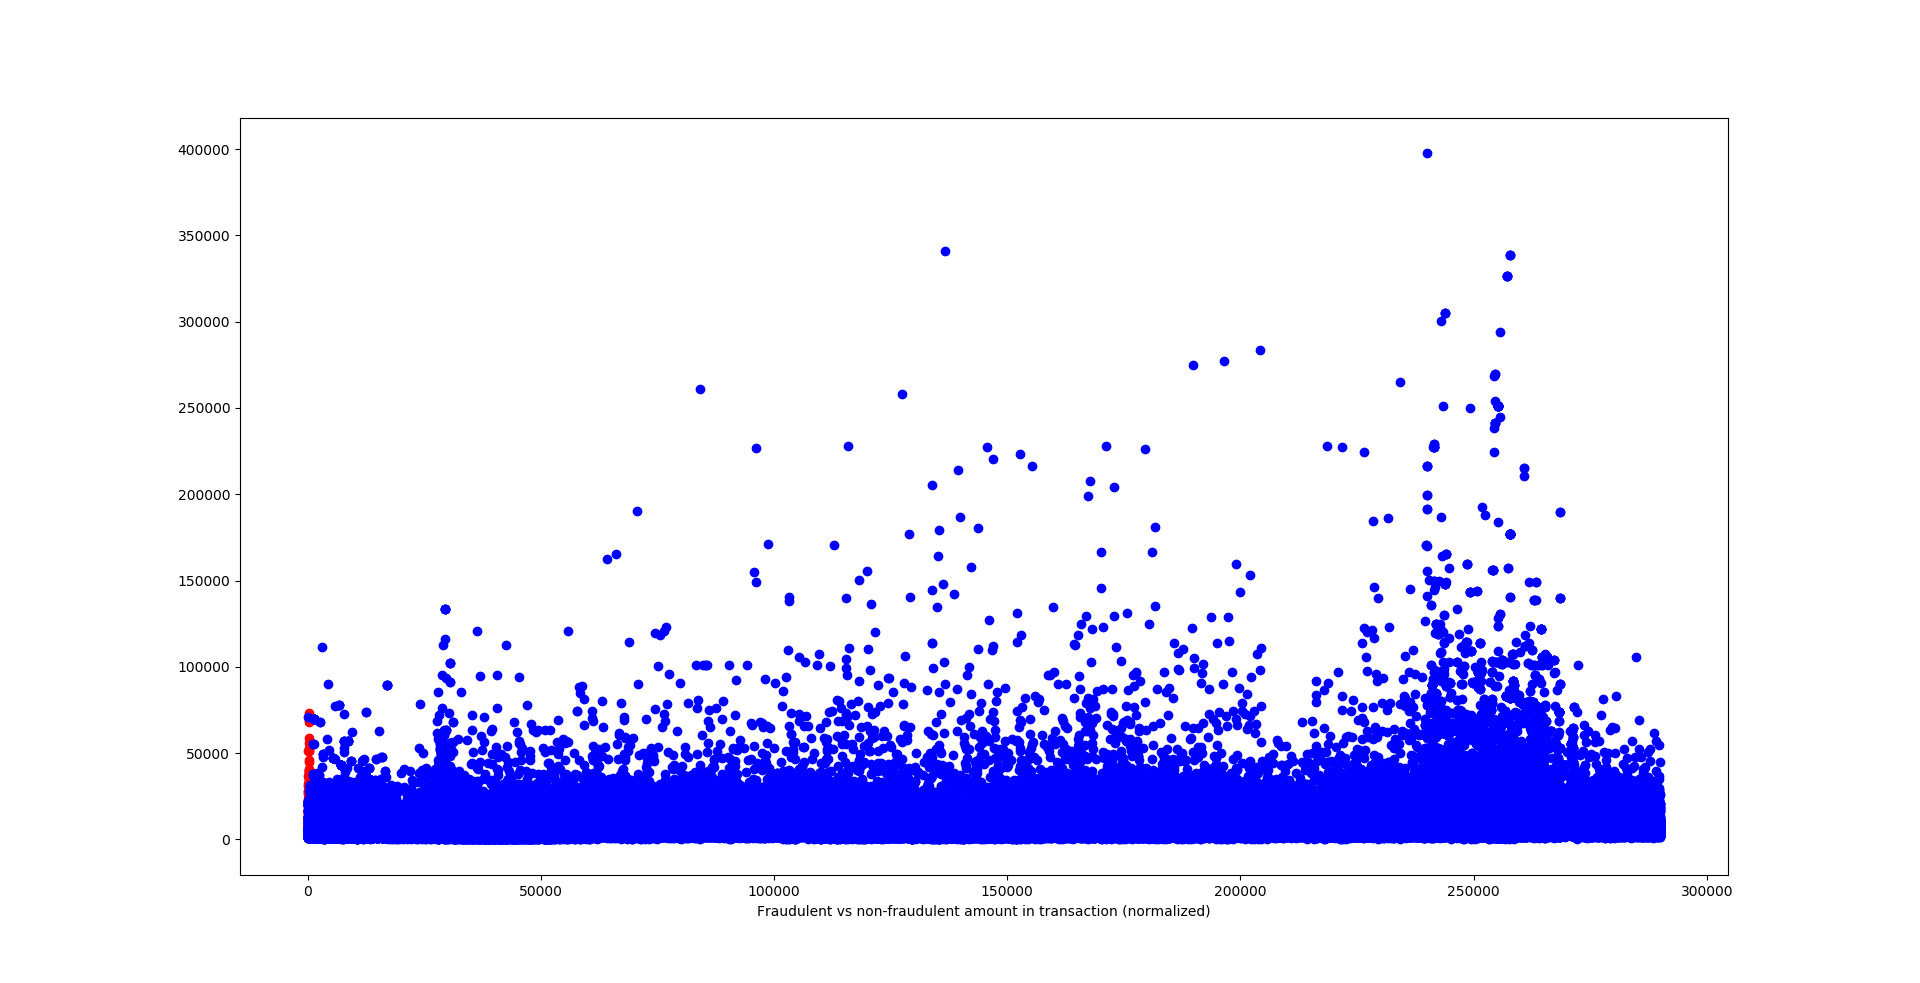
\includegraphics[scale = 0.25]{Visualizations/fraud_vs_nonfraud_better}
	\caption{A scatterplot of the amount of money spent in the sampled transactions. A red dot indicates a fraudulent transaction (these are only at the very left of the plot due to very little fraudulent transactions existing), while a blue dot indicates a benign transaction.}
\end{figure}
\clearpage
\section{Applying SMOTE to the data}
\end{document}
